\chapter{Appendix}

\section{Static Obstacle Collision checking}
\label{static_obst_appendix}
Static obstacle checking described in section \ref{osbtacle_check_satic} works on the concept that it is sufficient to check the lateral distance (D) between the obstacle and the ego at minimum and maximum of ego D (lateral coordinate) in the longitudinal intersection region.

Let $f(x)$ be a function of lateral motion D in intersection interval $[a,b]$, $f(x)\ge f(c)$ (respectively, $f(x)\le f(c)$), then $f(c)$ is the absolute minimum (respectively, absolute ) local maximum value of $f(x)$ on $[a,b]$ and vice versa. 

If $f(x)$ is continuous on $[a, b]$ and differentiable in $(a, b)$, a point $c$ in $[a, b]$ is a critical point of $f(x)$ if either $f'(c) =0$ or $f'(c)$ does not exist. The 

If $f(x)$ is continuous on $[a,b]$ and differentiable in (a,b), and if for some $c$ in $(a,b)$, if $f(c)$ is local minima or maxima then $c$ must be a critical point. Any absolute maximum or minimum will take place at boundaries or critical points inside the interval $(a,b)$. 


\begin{figure}[H]
	\centering
	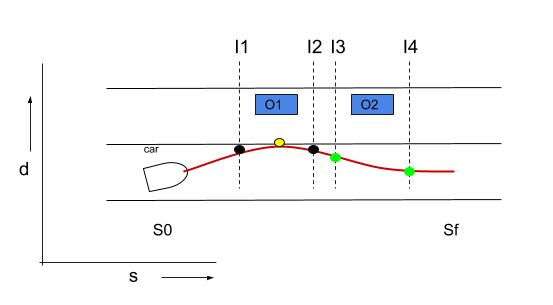
\includegraphics[width=0.8\textwidth]{Images/appendix/staticpoints.jpg}
	\caption{Static Obstacle Collision check - Lateral distance between obstacle O1 and trajectory is checked at points with black dots, distance at green dots is checked for obstacle O2.}
	\label{cstat_coll_appen}
\end{figure}

Consider $f(x) = x^3 - x^2 -x + 12$ with intersection interval in $[0,2]$, critical points are at $x=-1/3$ which is not in intersection and $x=1$ is in the intersection interval. Thus it is sufficient to check for values of $f(x)$ at [0,1,2] to find minima and maxima. 

In the figure \ref{cstat_coll_appen}, for obstacle O1 it is necessary to check collision at a critical point that lies in [I1, I2] represented with a yellow dot and at the borders represented with black dots. For the second obstacle O2, it is sufficient to check the boundaries of the interval [I3, I4]. If the critical points and the borders have an adequate lateral distance to the obstacle, then the rest of the points on trajectory will also have safe lateral distance, and it is not needed to check for collision at other points. 

%Proof thats its sufficient to check only at borders and only if global min or max exists in the intersection interval for collision checking with static obstacles
%https://www.math.wvu.edu/~hjlai/Words2Algebra/MinMax_Closed_Interva.pdf

\section{Dynamic Obstacle Collision checking}
\label{dynamic_obst_appendix}

In the proposed algorithm in section \ref{obstacle_check_dynamic}, for collision checking with respect to dynamic obstacles time difference only at the borders where lateral and longitudinal coordinates intersect is checked. This assumption is valid if the maximum non-linearity introduced by the ego vehicle acceleration is not more than 2s. The next set of equations define why the hypothesis is correct. 

Figure \ref{dynamic_approx_appen} shows where there is a difference between the linear approximation and the parabolic path. A black line shows the maximum time difference in the orange region. 

\begin{figure}
	\centering
	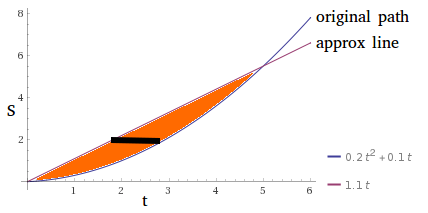
\includegraphics[width=0.8\textwidth]{Images/appendix/dynamic_approx.png}
	\caption{The parabolic curve indicates change of position with respect to time and the approx line indicates a linear change. The orange shared region indicates the maximum time difference between a linear approximated and the original curve. }
	\label{dynamic_approx_appen}
\end{figure}

Equation of the parabolic path. 
\begin{equation}
\label{curve_eq}
S_{curve} = ut + 0.5at^2
\end{equation}

Values of the function \ref{curve_eq} at start $0$ and time horizon $t_h = 5s$ 
\begin{equation}
S_0 = 0; S_f = 5u + 12.5a
\end{equation}

Corresponding approximated line equation $y=mx+c$, as both start at same point consider at origin. 
\begin{equation}
\label{line_eq}
S_{line} = \frac{5u+12.5a}{5}(t)
\end{equation}

Converting the \ref{curve_eq} as a function of distance, we get
\begin{equation}
t_{orig} = \frac{-u \pm \sqrt{u^2 + 2as}}{a}
\end{equation}

Converting the \ref{line_eq} as function of distance, we get
\begin{equation}
\label{line_eq}
t_{approx} = \frac{s}{u+2.5a}
\end{equation}

Time difference between original and approximated values is 

\begin{equation}
\label{t_diff_eq}
t_{diff} = \frac{-u \pm \sqrt{u^2 + 2as}}{a} - \frac{s}{u+2.5a}
\end{equation}

The maximum value of $t_{diff}$ between start and end of the path gives us the value required, as the equation is in 3 unknown variables, it is not possible to solve it directly to find the maximum value. Therefore exhaustive values are plotted to find the maximum value. The Figure \ref{time_diff_plot} shows the values of time difference for different values of acceleration from $-0.7ms^{-2}$ to $-0.3ms^{-2}$, initial velocity of $0ms^{-1}$ to $1ms^{-s}$ is used to plot in the region of $[0,u+12.5a]$ as s dimension. 


\begin{figure}[H]
	\centering
	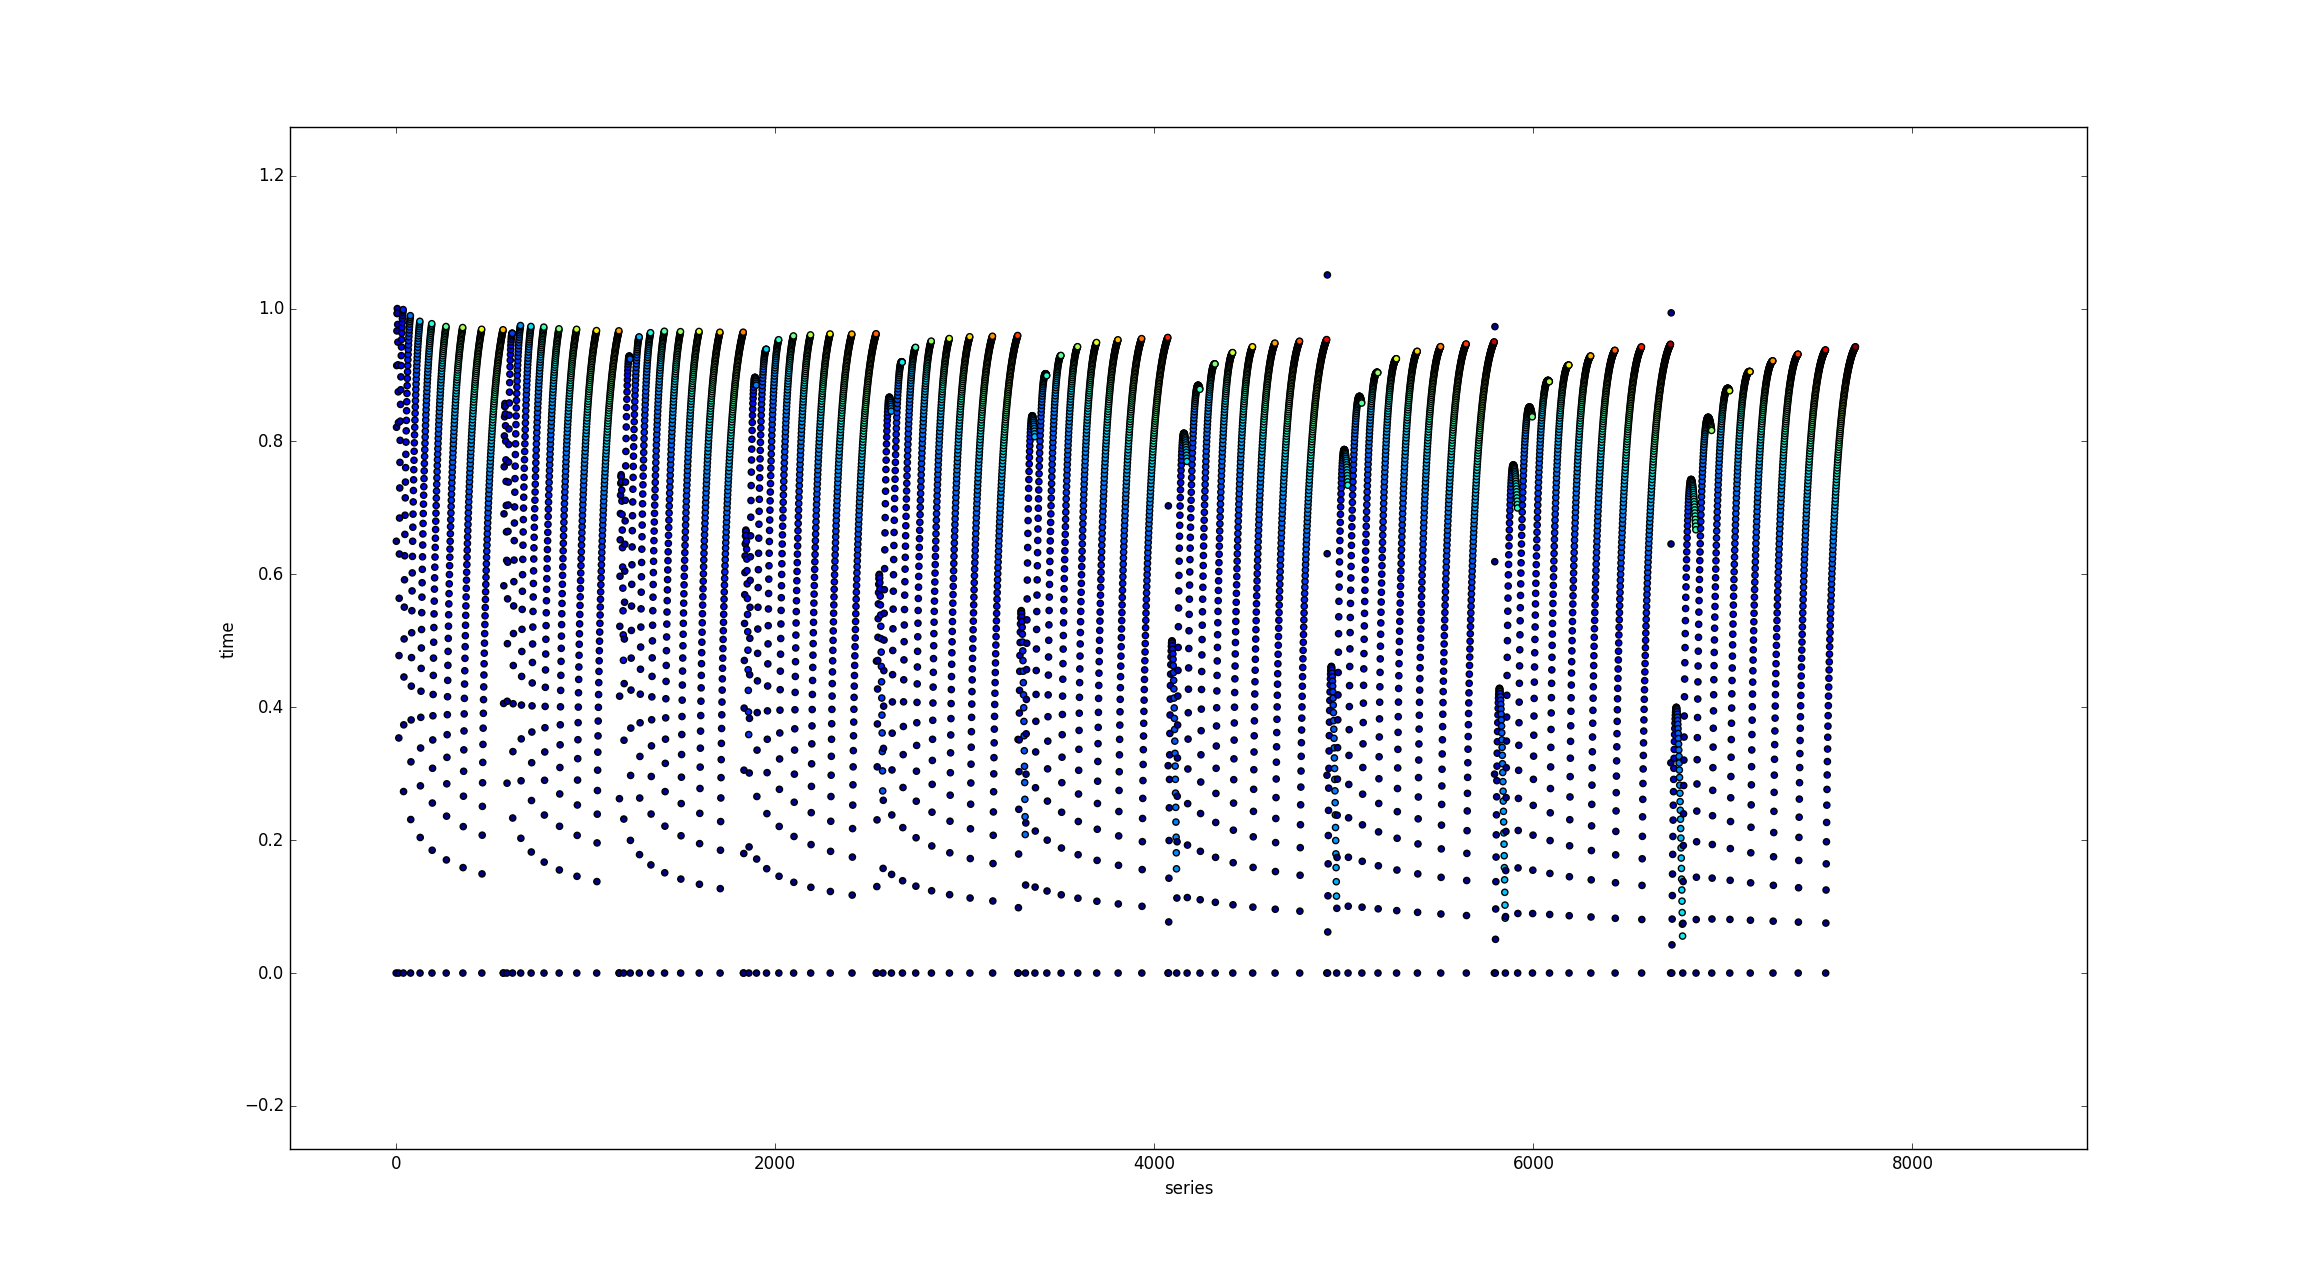
\includegraphics[width=1.0\textwidth]{Images/appendix/time_diff.png}
	\caption{Maximum time difference for different samples of different parameters of the equation \ref{t_diff_eq}}
	\label{time_diff_plot}
\end{figure}

The maximum difference at any point is 1s, thus the approximation holds good. The following python code is used to plot the results and find the maximum value.

\newpage
\begin{lstlisting}
from mpl_toolkits.mplot3d import Axes3D
import matplotlib.pyplot as plt
import numpy as np
from math import sqrt

def frange(start,stop, step=1.0):
	while start < stop:
		yield start
		start +=step
t = [] #time difference
r = [] #series number
co =[] #color differentiator
val =0 #series counter
for x in range(10):#u
	for y in range(10):#a
		k = 5*x+12.5*y #max distance range in multiple of 10
		if k<=0:
			k=0
		for z in  frange(0, k, 1):#s
			try:
				u=x/10.0
				a = -0.7+(y/1.0)
				s = z/10.0
				t_diff = ((-u+sqrt(u*u + 2*a*s))/a)-(s/(u+2*a))
				t.append(t_diff)
				r.append(val)
				co.append(z)
				val+=1
			except Exception as e:
				pass
plt.scatter(r,t,c=co)
plt.ylabel('time')
plt.xlabel('series')
plt.show()


\end{lstlisting}
